\begin{table*}[t]\centering
\caption{Measured efficiency. Train seconds exclude validation; threshold seconds include it. Throughput is in thousands of training samples/s. Peak allocated MiB includes GPU-resident development data.}
\label{tab:efficiency}\begin{tabular}{lrrrrr}\toprule
Method & Train (s) & Epoch (s) & k samples/s & Time to 85\% (s) & Peak (MiB)\\\midrule
SGD-M & \pmv{9.40}{0.21} & \pmv{0.63}{0.01} & \pmv{79.83}{1.80} & \pmv{1.43}{0.35} & \pmv{257.0}{0.0}\\
Adam & \pmv{11.31}{0.19} & \pmv{0.75}{0.01} & \pmv{66.31}{1.12} & \pmv{0.99}{0.42} & \pmv{258.3}{0.0}\\
AdamW & \pmv{11.16}{0.08} & \pmv{0.74}{0.01} & \pmv{67.20}{0.51} & \pmv{0.98}{0.43} & \pmv{258.3}{0.0}\\
Muon+AdamW & \pmv{22.04}{0.08} & \pmv{1.47}{0.01} & \pmv{34.03}{0.13} & \pmv{2.02}{1.00} & \pmv{257.8}{0.0}\\
\bottomrule\end{tabular}\end{table*}
\begin{figure*}[t]\centering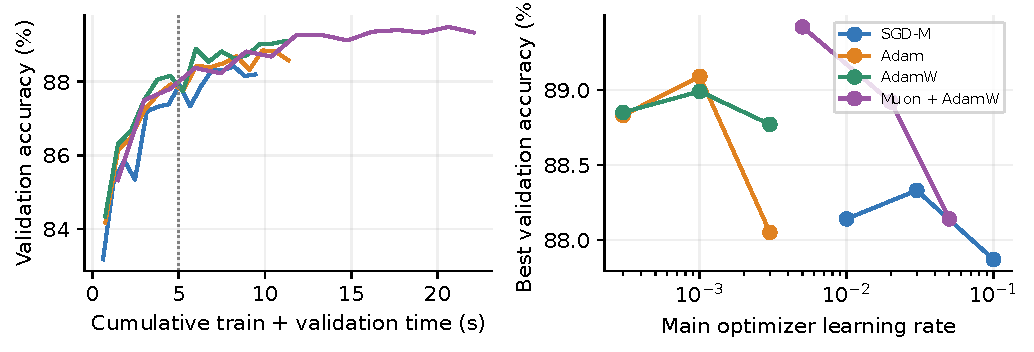
\includegraphics[width=.96\textwidth]{figures/efficiency_sensitivity.pdf}
\caption{Left: validation accuracy against measured cumulative training-plus-validation time; dotted line is the five-second budget. Right: validation-best accuracy for each of three learning-rate candidates (one tuning seed, ten epochs). Muon changes only its matrix learning rate; auxiliary AdamW stays at $10^{-3}$.}\label{fig:time}\end{figure*}
